% !TeX spellcheck = en_US
% !TeX encoding = UTF-8
% !TeX root = ../../thesis.tex

\chapter[%
    Introduction%
]{%
    Introduction%
    \footnote{
      Based on the authors' work in \cite{Sokolowski2024Automated,Sokolowski2024Pipr}.
    }
}
\label{sec:intro}

\Cref{sec:intro} is really about \lipsum[2]

Yay, an \Cref{sec:appA} \lipsum[5]

And a \Cref{fig:example} \lipsum[6]

\begin{figure}
  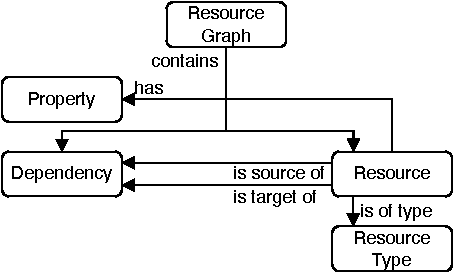
\includegraphics[width=.5\linewidth]{graphics/example.pdf}
  \caption{Example graphics.}
  \label{fig:example}
\end{figure}

And a \Cref{lst:example} \lipsum[6] \Cref{lin:example}

\begin{lstlisting}[
  caption={[Random Stuff.]%
      Random Stuff with a way too long caption.},
  label=lst:example,
  float]
rng.result.apply((wordId) => {
  new aws.s3.BucketObject('index', {
      bucket: bucket, key: 'index.html',
      contentType: 'text/html; charset=utf-8',
      content: '<!DOCTYPE html>' +
               words[wordId].toUpperCase()
  });~\label{lin:example}~
});
\end{lstlisting}

Table stuff going in \Cref{tab:example} \lipsum[6]
\begin{table}
	\caption{Weird table title example.} 
	\label{tab:example}
	\begin{tabular}{lr}
		\toprule
		\multicolumn{2}{c}{Channel \hspace{2cm} Responses} \\ 
		\midrule
		DevOps Chat Slack & 3 \\ 
		Devops Weekly Newsletter & 24  \\ 
		Facebook & 3 \\ 
		LinkedIn & 7 \\ 
		\bottomrule
	\end{tabular}
\end{table}


\section{Publications}
\label{sec:intro:publications}

\newcommand{\ownPub}[1]{\item[\cite{#1}] % get/setmaxcitenames dance ensures that all authors are printed
    \numdef{\origmaxcitenames}{\getmaxcitenames{}}\setmaxcitenames{99}\fullcite{#1}\setmaxcitenames{\origmaxcitenames}}
\newcommand{\ownPubUsed}[2]{\ownPub{#1} \newline [Used in #2]}

This dissertation led to the following publications at peer-reviewed journals, conferences, and workshops.
Their content is used verbatim in this dissertation as stated below.

\begin{itemize}[leftmargin=3em]
    \ownPubUsed{Sokolowski2024Automated}{\Cref{sec:intro}}
\end{itemize}

\noindent
Beyond the publications constituting this dissertation,
I (co)authored the following peer-reviewed articles during my doctoral studies.

\begin{itemize}[leftmargin=3em]
  \ownPub{Sokolowski2024Pipr}
\end{itemize}